% !TeX root = ../main.tex

\chapter{空空导弹任务分配模型}
\label{chap:model}

%----------------------------
\section{引言}
\label{model:sec:intro}

在任务分配问题中,首先需要根据导弹自身传感器或其他支持平台收集得到的数据和信息,估计战场态势,建立多对多的任务分配模型。在空空导弹的作战场景下,本节选择了预计剩余攻击时间和当前导弹机动量是两个较为显著且易于获得的影响要素,首先分别介绍了两个要素的估计方法,之后以最小化总攻击时间和最小化导弹机动量为目标函数,建立多对多任务分配模型。


\section{弹目相对运动模型}
\label{model:sec:move}

\begin{figure}[htp]
  \centering
  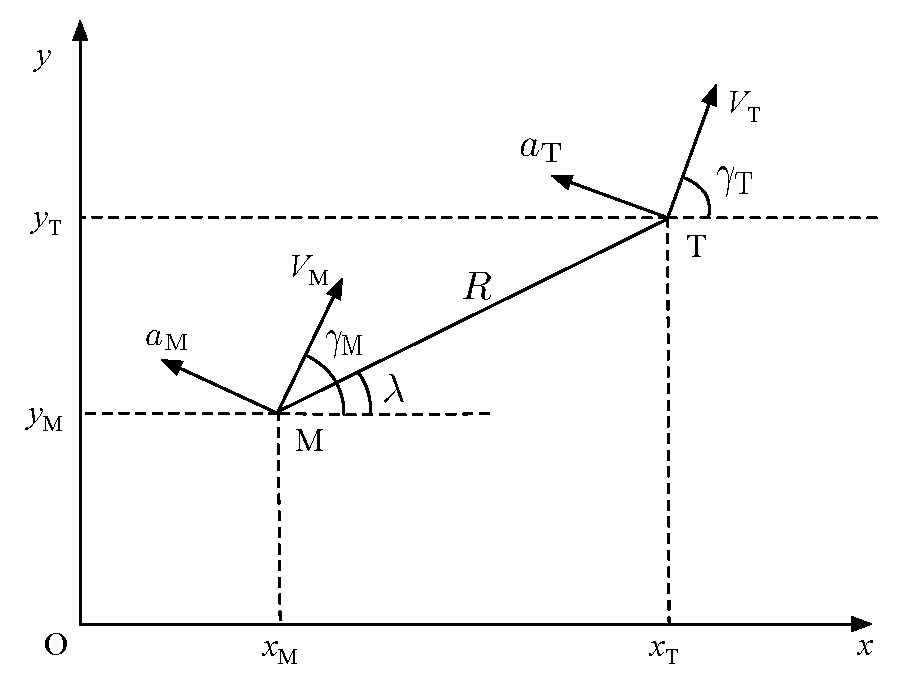
\includegraphics[width=10cm]{model.eps} \\
  \bicaption[弹目相对运动模型]
    {弹目相对运动模型}
    {Relative motion model of missile and target}
 \label{fig:model}
\end{figure}

在建立多对多任务分配模型之前,需要先建立一对一的空战模型本文所考虑的模型是在二维平面内,不考虑导弹和目标具体形状的影响,即将导弹和目标当作质点处理。图\ref{fig:model}展示的是本文所使用的导弹与目标相对运动模型,其中M表示导弹,T表示目标,$[x_{(\cdot)},y_{(\cdot)}],V_{(\cdot)},a_{(\cdot)},\gamma_{(\cdot)}$分别表示导弹和目标的位置、速度、加速度和航向角。$r$为弹目距离,$\lambda$表示弹目视线角。

为了建立弹目相对运动模型,需要作出以下假设:1、导弹与目标速度均为常值;2、目标的速度小于导弹的速度。由此分别建立导弹和目标的运动方程为:

\begin{align}
	\label{model:eq:Mmotion} \dot{x_{\text M}}&=V_{\text M} \cos{\gamma_{\text M}},\ \dot{y_{\text M}}=V_{\text M} \sin{\gamma_{\text M}},\ \dot{\gamma_{\text M}}=\dfrac{a_{\text M}}{V_{\text M}},\\
	\label{model:eq:Tmotion} \dot{x_{\text T}}&=V_{\text T} \cos{\gamma_{\text T}},\ \dot{y_{\text T}}=V_{\text T} \sin{\gamma_{\text T}},\ \dot{\gamma_{\text T}}=\dfrac{a_{\text T}}{V_{\text T}}.
\end{align}

令$V_R,V_{\lambda}$分别表示弹目相对速度平行于和垂直于视线角方向的分量,$V_R$表示弹目相对接近速度,则弹目相对运动方程为:

\begin{align}
	\label{model:eq:Rrelative} V_R & \equiv \dot{R}=V_{\text T}\cos{\sigma_{\text T}}-V_{\text M}\cos{\sigma_{\text M}},\\
	\label{model:eq:Lrelative} V_{\lambda} & \equiv R\dot{\lambda} = V_{\text T}\sin{\sigma_{\text T}}-V_{\text M}\sin{\sigma_{\text M}},
\end{align}
其中$\sigma_{(\cdot)},\ (\cdot) \in \{\text M,\text T\}$分别表示是导弹和目标的前置角,其定义为:

\begin{equation}
\label{model:eq:forwardAngle}
	\sigma_{\text M} = \gamma_{\text M}-\lambda,\quad \sigma_{\text T}=\gamma_{\text T}-\lambda.
\end{equation}

由此可求得视线角变化率:

\begin{equation}
\label{model:eq:dotlambda}
	\dot \lambda = \frac{V_{\text T}\sin{\sigma_{\text T}}-V_{\text M}\sin{\sigma_{\text M}}}{R}.
\end{equation}


% --------------------------------
\section{剩余攻击时间估计}
\label{model:sec:time}

在导弹攻击过程中,为了使得预计击中时间最短,需要估计剩余攻击时间,本节采用对目标状态投影到弹目视线方向,将目标转化为相对静止状态的思想,实现对机动目标的剩余攻击时间估计。

首先假设目标静止,即$V_{\text T}=0$。此时由式(\ref{model:eq:Mmotion})、(\ref{model:eq:forwardAngle})和(\ref{model:eq:dotlambda})可得:

\begin{equation}
\label{model:eq:dotsigma}
	\dot{\sigma_{\text M}}=\frac{a_{\text M}}{V_{\text M}}+\frac{V_{\text M}\sin{\sigma_{\text M}}}{R},
\end{equation}

结合式(\ref{model:eq:Rrelative})可得:

\begin{equation}
\label{model:eq:sigmaDotR}
	\frac{d\sigma_{\text M}}{dR} = -\frac{a_{\text M}}{V_{\text M}^2\cos{\sigma_{\text M}}}-\frac{1}{R}\tan{\sigma_{\text M}}.
\end{equation}

为方便叙述,令$\rho=\sin{\sigma_{\text M}}$,代入式(\ref{model:eq:sigmaDotR})可得:

\begin{equation}
\label{model:eq:rhoDotR}
	\frac{d\rho}{dR} = -\frac{a_{\text M}}{V_{\text M}^2}-\frac{1}{R}\rho.
\end{equation}

此处为方便推导,考虑导弹采用比例制导律,制导指令为:

\begin{equation}
\label{model:eq:png}
	a_{\text M}=N V_{\text M} \dot{\lambda},
\end{equation}
其中$N$为制导比例系数。将式(\ref{model:eq:png})和(\ref{model:eq:dotlambda})代入式(\ref{model:eq:rhoDotR})可得:

\begin{equation}
\label{model:eq:rhoDotR2}
	\frac{d\rho}{dR} = (N-1)\frac{\rho}{R}.
\end{equation}

式(\ref{model:eq:rhoDotR2})是一个一阶微分方程,其解形式为:

\begin{equation}
\label{model:eq:rho}
	\rho=\rho_0 \Bigg(\frac{R}{R_0}\Bigg)^{N-1},
\end{equation}
其中$\rho_0$和$R_0$分别为初始时刻的对应变量值。将式(\ref{model:eq:Rrelative})两边对$R$求积分,并进行泰勒展开得到:

\begin{align}
\label{model:eq:terminalTime}
	t_f &= \frac{1}{V_{\text M}} \int_0^{R_0} \frac{1}{\sqrt{1-\rho^2}}dR \notag \\
	&= \frac{1}{V_{\text M}} \int_{0}^{R_0} \Big(1+\sum_{i=1}^{\infty} \frac{2i-1}{2^i}\rho^{2i} \Big)dR,
\end{align}
其中$t_f$为初始时刻导弹已经飞行的时间。为简化问题,仅取式(\ref{model:eq:terminalTime})泰勒展开的前两项代入式(\ref{model:eq:rho})求解,并使用小角度假设$\rho \approx \sigma_{\text M}$可得:

\begin{equation}
\label{model:eq:tfsolution}
	t_f = \frac{R_0}{V_{\text M}} \Big(1+\frac{1}{2(2N-1)}\sigma_{\text M0}^2 \Big).
\end{equation}

因此,若在每个时刻均取该时刻视线角方向作为$x$轴,则可得目标静止时在每个时刻的剩余攻击时间的估计值为:

\begin{equation}
\label{model:eq:stillTF}
	t_{\text{go}} = \frac{R}{V_{\text M}} \Big(1+\frac{1}{2(2N-1)}\sigma_{\text M}^2 \Big).
\end{equation}

针对机动目标对式(\ref{model:eq:stillTF})作出进一步修正,采用虚拟目标的思路,将$V_{\text T}$和$a_{\text T}$对弹目相对运动的影响均投影到弹目视线角方向上,并修正由目标机动引起的航向角和视线角变化,将目标转化为相对静止状态。

首先得到目标机动引起的目标航向角和视线角的变化分别为:

\begin{equation}
\label{model:eq:diffsigma}
	\hat \sigma_{\text T} = \frac{a_{\text T}}{V_{\text T}}\cdot \hat t_{\text{go}}^p,\quad \hat \lambda=\frac{V_{\text T}\sin{\sigma_{\text T}}}{R}\cdot \hat t_{\text{go}}^p,
\end{equation}
其中$\hat t_{\text{go}}^p$表示前一时刻对$t_{\text{go}}$的估计值,修正后的剩余攻击时间估计为:

\begin{equation}
\label{model:eq:modifiedTF}
	\hat t_{\text {go}} = \frac{R}{V_{\text{MT}}}\Big(1+\frac{1}{2(2N-1)}\sigma_{\text M}^2 \Big)
\end{equation}
其中$V_{\text{MT}}=V_{\text M}-V_{\text T}\cos(\sigma_{\text T}+\hat \sigma_{\text T}-\lambda-\hat \lambda)$。


% --------------------------------------------
\section{最优制导律}
\label{model:sec:energy}

除了预计攻击时间最小化以外,由于导弹在攻击过程中大部分时间处于无动力滑翔阶段,在机动追踪目标时会不断消耗能量,因此为了保证击中目标前导弹动能不会耗尽,需要追求导弹机动程度最小化。实际中导弹系统具有高阶动态特性和非线性,难以利用最优控制原理求得闭环解,但对于只考虑导弹低阶系统特性和二次型性能指标取极小的最优控制问题,可以求得闭环解。本节将在导弹在\ref{model:sec:time}小节估计剩余攻击时间的基础上,基于最优控制原理,设计使得导弹机动最小化的最优制导律。

首先假设目标不机动,即$a_{\text T}=0$将\ref{model:sec:move}节建立的弹目相对运动模型改写为惯性系下的状态方程形式:

\begin{align}
\label{model:eq:state}
	\dot{\bm{x}} = \bm{Ax}+&\bm{Bu},\\
	\bm{A} = \begin{bmatrix}
		0 & {\bm I}_2 & 0\\
		0 & 0 & {\bm I}_2\\
		0 & 0 & -\frac{1}{\tau}{\bm I}_2\\
	\end{bmatrix},\ 
	&\bm{B} = \begin{bmatrix}
		0\\0\\\frac{1}{\tau}{\bm I}_2
	\end{bmatrix},
\end{align}
其中状态向量为${\bm x}=[{\bm R}^{\mathrm T},{\dot{\bm R}}^{\mathrm T},{\bm a}_{\text M}^{\mathrm T}]^{\mathrm T}$,各状态分量分别为对应变量的向量形式,${\bm I}_2$为二阶单位矩阵,$\tau$为导弹的等效时间常数。

设二次型的性能指标为

\begin{alignat}{2}
	\label{model:eq:J} \min \quad & J = \frac{1}{2}\int_{t_0}^{t_f} {\bm u}^{\mathrm T} {\bm u} dt,\\
	\mbox{s.t.} \quad 
	\label{model:eq:Jconstraint} & R(t_f)=0.
\end{alignat}

其中$t_0$和$t_f$分别表示制导开始和结束的时间,式(\ref{model:eq:J})可减小机动能量的消耗,有利于保持弹道平直,减小损耗增大射程。式(\ref{model:eq:Jconstraint})可约束末端脱靶量为0。

上述最优控制问题可求解闭环最优控制率形式为

\begin{equation}
\label{model:eq:closedU}
	u = ({\bm B}^{\text T}{\bm P}k^{-1})M,
\end{equation}
其中$k$是当$u=0$时的预计末端脱靶量,可由下式求得:

\begin{equation}
\label{model:eq:M}
	M={\bm P}^{\mathrm T}{\bm X}.
\end{equation}

由下列微分方程
\begin{align}
\label{model:eq:ricati}
	\dot{\bm P} + {\bm A}^{\mathrm T}{\bm P} = 0,\ {\bm P}(t_f)=\begin{bmatrix}
		1\\0\\0
	\end{bmatrix},
\end{align}
可求得$\bm P$的闭环表达式为
\begin{equation}
\label{model:eq:P}
	{\bm P} = \begin{bmatrix}
		1\\t_{\text{go}}\\\tau^2(e^{-T}+T-1)
	\end{bmatrix},
\end{equation}
其中$t_{\text{go}}$是预计剩余攻击时间,$t_{\text{go}}=t_f-t$,$T=t_{\text{go}}/\tau$。由

\begin{equation}
\label{model:eq:k}
	k = -\int_{t}^{t_f} ({\bm P}^{\mathrm T}{\bm G}{\bm G}^{\mathrm T}{\bm P}) dt,
\end{equation}
可求得$k$等于
\begin{equation}
\label{model:eq:ksolution}
	k = \tau^3(\frac{1}{2}e^{-2T} + 2Te^{-T} - \frac{T^3}{3} + T^2 - T - \frac{1}{2}).
\end{equation}

将式(\ref{model:eq:P})和式(\ref{model:eq:ksolution})代入式(\ref{model:eq:closedU})和式(\ref{model:eq:M})求得最优制导律闭合解为

\begin{equation}
\label{model:eq:oplStill}
	u = \frac{N'}{t_{\text{go}}^2} [ \bm R+\dot{\bm R}t_{\text{go}} - \tau^2(e^{-T}-1+T) {\bm a}_{\text M}],
\end{equation}
其中$N'$为扩展比例系数:

\begin{equation}
\label{model:eq:oplparameters}
	N' = T^2 (e^{-T}-{\bm I}_2+T) (-\frac{1}{2}e^{-2T} - 2Te^{-T} + \frac{1}{3}T^3 - T^2 + T + \frac{1}{2}{\bm I}_2)^{-1}.
\end{equation}

在目标机动的情况下,可对式(\ref{model:eq:oplStill})进行修正,限于篇幅,这里不再展开,直接给出对于机动目标的最优制导律:

\begin{equation}
\label{model:eq:oplMove}
	u = \frac{N'}{t_{\text{go}}^2} [ \bm R+\dot{\bm R}t_{\text{go}} - \tau^2(e^{-T}-1+T) {\bm a}_{\text M}-\frac{t_{\text{go}}^2}{2}a_{\text T}].
\end{equation}

最优性能指标$J^*$为

\begin{equation}
\label{model:eq:Jstar}
	J^* = \frac{1}{2} {\bm X}^{\mathrm T}(t_0) {\bm P}(t_0) {\bm P}^{\mathrm T}(t_0) {\bm X}(t_0).
\end{equation}

%---------------------------------------------
\section{任务分配模型建立}
\label{model:sec:assignment}

假设我方有$n_m$枚导弹,其集合表示为$\mathcal{M} := \{\mathcal{M}_1,\dots,\mathcal{M}_{n_v}\}$;战场上有$n_t$个目标需要攻击,其集合表示为$\mathcal{T} := \{\mathcal{T}_0,\mathcal{T}_1,\dots,\mathcal{T}_{n_t}\}$,其中$\mathcal{T}_0$表示空目标。本文只考虑导弹数量不少于目标数量,即$n_m \geq n_t$的情况。每枚导弹可根据自身能力、所处环境等因素选择部分目标作为可攻击对象,设$\mathcal{A}_i \subset \mathcal{T}$表示第$i$枚导弹的可选目标集。特别地,为后续叙述方便,假设$\mathcal{T}_0 \in \mathcal{A}_i,\ i=1,\dots,n_m$,即所有导弹总是可以选择不攻击任何目标。\footnote{显然,根据实际场景以及约束条件可知导弹不攻击任何目标是不符合实际要求的,本文在此作出的假设仅仅是为了后面章节叙述和论证需要,无任何实际意义,对问题的论述和求解也无任何影响。}导弹$i$从自己的可选目标集$\mathcal{A}_i$中选出自己的目标$a_i$,则数组$a=(a_1,\dots,a_{n_m})\in \mathcal{A}$组成了一个分配解。设$S(a)=\{S_1,\dots,S_{n_t}\}$,其中$S_j$表示分配解$a$下选择目标$j$的导弹集合,$s_j$表示$S_j$中的导弹个数,即$s_j = |S_j|, j=1,\dots,n_t$。

选取一个关于分配解$a$的函数$U_g(a)$作为全局效用函数,建立任务分配模型:

\begin{alignat}{2}
	\label{model:eq:globalU} \max_{a \in \mathcal{A}} \quad & U_g(a) = \sum_{\mathcal{T}_j \in \mathcal{T}} U_{\mathcal T_j}(a)\\
	\mbox{s.t.} \quad 
	\label{model:eq:bmax} & s_j \leq b_{\text{max}}^{(j)},\ j=1,\dots,n_t\\
	\label{model:eq:bmin}& s_j \geq 1,\ j=1,\dots,n_t,
\end{alignat}
其中$b_{\text{max}}^{(j)}$表示选择目标$j$的导弹的最大数量和最小数量,且有$b_{\text{max}}^{(j)} \geq 1$。因此式(\ref{model:eq:bmax})表示目标$j$不得被超过$b_{\text{max}}^{(j)}$枚导弹攻击,式(\ref{model:eq:bmin})代表每个目标必须有导弹攻击,但由于实际中往往使用多于目标数量的导弹攻击,因此在式(\ref{model:eq:bmin})的约束下,式(\ref{model:eq:bmin})自然成立,因此可将上述问题进一步简化为

\begin{alignat}{2}
	\label{model:eq:simUg} \max_{a \in \mathcal{A}} \quad & U_g(a) = \sum_{\mathcal{T}_j \in \mathcal{T}} U_{\mathcal T_j}(a)\\
	\mbox{s.t.} \quad 
	\label{model:eq:simbmax} & s_j \leq b_{\text{max}}^{(j)},\ j=1,\dots,n_t.
\end{alignat}

$U_{\mathcal T_j}(a)$表示与目标$\mathcal{T}_j$有关的任务效用,为了体现预计剩余攻击时间最小和导弹机动能量消耗最小的目标,利用\ref{model:sec:time}小节和\ref{model:sec:energy}小节的内容,将任务效用函数设计为:

\begin{equation}
\label{model:eq:taskU}
	U_{\mathcal{T}_j}(a) = \max \{ 0, r_j - w_1 \max_{\mathcal{M}_i \in S_j} t_{ij} -
	w_2 \mathcal{C}_{\mathcal{T}_j} \},
\end{equation}
其中,$w_1$和$w_2$为权重值;$r_j$是攻击目标$\mathcal{T}_j$可获得的奖励值,本文假设该值仅与目标属性有关,与攻击的导弹无关;$t_{ij}$表示导弹$\mathcal{M}_i$攻击目标$\mathcal{T}_j$的预计剩余攻击时间。$\mathcal{C}_{\mathcal{T}_j}$表示导弹攻击目标$\mathcal{T}_j$的成本函数,定义为:

\begin{equation}
\label{model:eq:costU}
	\mathcal{C}_{\mathcal{T}_j} = \sum_{\mathcal{M}_i \in S_j} J_{ij},
\end{equation}
其中$J_{ij}$为导弹$\mathcal{M}_i$攻击目标$\mathcal{T}_j$的预计机动能量消耗可由式(\ref{model:eq:Jstar})得到。

\section{本章小结}
\label{model:sec:conclusion}
本章基于攻击时间最小化和导弹机动消耗最小化的原则建立了空空导弹任务分配模型。首先建立了弹目相对运动模型,对导弹和目标的运动方程进行建模。接着基于该相对运动模型估计剩余攻击时间,并设计导弹遵循最优制导律飞行已获得最小机动消耗。最后,本章定义了全局效用函数和任务效用函数的概念,建立了导弹与目标的任务分配模型,为后续求解空空导弹的任务分配问题打下基础。














